\documentclass{article}
\usepackage[utf8]{inputenc}
\usepackage[margin=1.25in]{geometry}
\usepackage{mivanit_texstyle}
\usepackage{amssymb,amsthm,enumitem,graphicx,mathtools,titling,tikz}

%% Define custom enumerate environment for deeper nesting
%\newlist{myEnumerate}{enumerate}{5}
%\setenumerate{listparindent=\parindent}
%\setlist[myEnumerate,1]{label=(\arabic*)}
%\setlist[myEnumerate,2]{label=(\alph*)}
%\setlist[myEnumerate,3]{label=(\roman*)}
%\setlist[myEnumerate,4]{label=(\alph*)}
%\setlist[myEnumerate,5]{label=(\roman*)}
%\setlistdepth{7}

%\newcommand{\ben}{\begin{myEnumerate}}
%\newcommand{\een}{\end{myEnumerate}}

\newcommand{\tensProd}{\otimes}
\newcommand{\graphSum}{\oplus}

\newcommand{\M}{\mathbb{M}}

%\makeatletter\newcommand{\skipitems}[1]{%
%  \addtocounter{\@enumctr}{#1}%
%  }\makeatother

%% Increases spacing between lines
\renewcommand{\baselinestretch}{1.175}

%% Shrink spacing between text and environments
\expandafter\def\expandafter\normalsize\expandafter{%
    \normalsize
    \setlength\abovedisplayskip{4.5pt}
    \setlength\belowdisplayskip{4.5pt}
    \setlength\abovedisplayshortskip{4.5pt}
    \setlength\belowdisplayshortskip{4.5pt}}

%% Adjust sizing and spacing of header
%\pretitle{\begin{center}\huge}
%\posttitle{\par\end{center}}
%\preauthor{\begin{center}\large}
%\postauthor{\end{center}}
\date{}

\title{TITLE}
\title{Spiking Neural Networks as a Model for the Nervous System of \textit{Hydra}}
\begin{document}
\maketitle

\section{Introduction}

An artificial neural network is a simplification of a biological neural network, generally based on a directed weighted graph. The vertices of the graph represent neurons, and the edges represent connections between them. Typically, these artificial neurons are only vaguely inspired by biological neurons, and therefore are unsuitable for use in modeling biological nerve networks. We hope to work past some of the biological limitations of traditional artificial neural networks using what are known as spiking neural networks, and aim to apply them in creating a model of the very primitive nervous system of the metazoans \textit{Hydra}.

%We aim to compare the structure and learning techniques of artificial and biological neural networks, and then attempt to construct artificial models that better mimic biological nerve nets, specifically that of \emph{Hydra}. Firstly, we hope to investigate ways to imitate chemical signalling in artificial neural networks, as they appear to play an important role in both learning and emotions in the human brain, and nothing similar in function exists in most artificial neural networks. Secondly, we hope to construct a threshold-based and always-running artificial neural network that we will attempt to train to complete simple tasks. To do this, we will use a novel approach involving the use of graph tensor products to reduce the memory requirements for large neural networks.

\section{The nervous system of \textit{Hydra}}
\textit{Hydra} is a genus of small, freshwater cnidarians which have long been studied in laboratories, due to both their ease of culturing and small size (typically 10 mm in length). They have one of the simplest nervous systems known among metazoans, yet they are still capable of nontrivial behaviors, unlike more basal clades such as \textit{Porifera} (sponges). Due to this simplicity, as well as the large knowledge base surrounding \textit{Hydra}, we aim to develop a basic model of the \textit{Hydra} nervous system.

Like other cnidarians, \textit{Hydra} do not have a central nervous system, but rather a nerve net, which is characterized by neurons distributed throughout the body with little centralization (i.e. no brain). That said, the neurons are still not distributed homogeneously across the body of \textit{Hydra}, but assuming as much is a decent approximation. Extending our model to consider more complex neuronal distributions would be an interesting topic for further exploration.

Being such primitive organisms, \textit{Hydra} have a very limited set of behaviors. \textit{Hydra} are capable of movement, but they are primary sessile, with their primary behaviors being elongation and contraction. Interestingly, Han et al., 2018, examined freely behaving \textit{Hydra} and found that the specific set of behaviors observed is independent of environmental conditions. Dupre and Yuste, 2017, completed the first ever full nervous system activity map using \textit{Hydra}, and found that the primary behaviors of \textit{Hydra} are controlled by disjoint circuits in the nerve net. That is, each neuron belongs to a single connected group of neurons (a circuit), and each circuit controls a specific behavior. However, at least two of the circuits have an antagonistic relationship, so they are not completely independent of each other.

We plan to use a spiking neural network as the basis for our model. Unfortunately, we do not have any numerical data to use, so we will have to train the network on estimated data points. The exact values should not matter as long as orders of magnitude are consistent across the data set – all that should matter is correlation. For example, as mechanical pressure is applied to the tentacles, the \textit{Hydra} should contract longitudinally (as observed experimentally), and this negative correlation should be reflected in the data set.

%\section{Assumptions}
%\subsection{Threshold v.s. Continuous activation}
%In modern artificial neural networks, a neuron's output edges have an output strength dependent on the input strength, usually through a sigmoid function. This is in contrast to biological neural networks. As we learned in class, a neuron will fire if and only if the voltage passes a certain threshold. The usual explanation for this given in the literature is that a smooth function works better for the types of gradient ascent used in learning, namely back-propagation. One of our goals is to get data on the difference between the learning speeds of neural networks that use a threshold model (step function) or some other activation function.

\section{Spiking Neural Networks}
Traditional neural networks used today in deep learning have their neurons fire only during what is known as a propagation cycle. That is, if the neural network is to act as an agent in some environment, then the timesteps must be discrete. On one hand, making the simplification that neurons fire only during a propagation cycle makes the simulation of networks much easier, and is perfectly fine for applications such as image recognition. However, it is far less realistic when trying to simulate an actual biological nervous systems which runs on a continuous time scale.

Spiking neural networks aim to solve this problem in part. Firstly, this type of neural network includes continuous time as a factor in the model. This leads artificial neurons to behave more like biological neurons, only firing once a predetermined 'membrane potential' has been reached. If the input is not strong enough, the current potential will degrade over time. If the neuron fires, the signal travels to other neurons but not instantaneously as in traditional networks. Finally, a refractory period can be added so that the neuron does not fire immediately after having fired, giving it a sort of cool down period as is observed in biological neurons. All these properties together make spiking neural networks a better choice for our model than any other traditional neural network design.

\section{Appendix: Optimization through graph tensor products}

We assume that the graph structure of a biological neural network at some time $t$ can be modeled by a time dependent function $\M$ that transforms the edge and vertex sets of an initial graph $G$ in some fashion. Further, we will model networks under the assumption that the initial structure of $G$ before any edge weights are modified can be approximated by the tensor product of other graphs:

$$ G = (H_1 \tensProd H_2 \tensProd \cdots \tensProd H_L ) $$

The reason for this assumption is as follows. For the tensor product $ C = A \otimes B$ of two graphs $A,B$ with $|V_A| = h, |V_B| = k$, the size of the vertex set of $C$ is $h \cdot k$. However, we can simulate a random walk on $C$ with only $(h + k)$ memory for the vertices, despite the vastly increased complexity of the graph. This is a fundamental property of graph tensor products. For our applications, of course, we are not trying to simulate a random walk, but there are computational savings nonetheless. See section \ref{code_outline} for more details.

An important distinction is that a neural networks changes with time as it learns, and this is where our function $\M : (G, t) \mapsto G_t$ comes into play. In most artificial feed-forward neural networks, the function would simply modify the weights of the edges of $G$ in accordance to some fitness function. However, for our purposes, modification of the underlying product components $\listvec{H}{L}$ may be advantageous, particularly in the early stages of learning. This is because modifications to the underlying product components create large changes in the structure of the network at little computational expense.

\subsection{Code notes} \label{code_outline}
\begin{itemize}
    \item When storing the graph $G$, we store the tensor product components $\listvec{H}{L}$ where $L$ is the number of layers. To specify a vertex $v$ in $G$, we store in an $L$-element array the vertices $v_i \in H_i$ to which $v$ corresponds to.

    \item To store an edge $e$ that is an addition to $G$ or the change of an existing edge weight in $G$s we store the vertices $v_1, v_2$ which it connects, and store the edge in a data structure sorted by the input vertex $v_1$. Given a vertex $v_1$, this lets us easily access the edges leading away from $v_1$.

    \item To avoid having the repetitive weights from the original graph $G$, the weights of $M(G,0)$ are determined by hash function until the vast majority of edges are changed, and then we begin to store the edges directly.

\end{itemize}
%priority queue for vertices?
%\section{Challenges}
%difficult to choose good initial $\listvec{H}{L}$


\section{Artifical Neural Networks}
%%%%%%%%%%%%%%%%%%%%%%%%%%%%%%%%%%%%%%%%%%%%%%%%%%%%%%%%%%%%%%%%%%%%%%%%%
%%%%%%%%%%%%%%%%%%%%%%%%%%%%%%%%%%%%%%%%%%%%%%%%%%%%%%%%%%%%%%%%%%%%%%%%%

\subsection{Artificial Neural Network (ANN) Introduction}
\begin{itemize}
\item Neurons represented by vertices in a weighted directed graph
\item Output of a neuron is a function of the weighted sum of inputs
\item Usually have multiple hidden layers of neurons
\item Learning accomplished through modifying edge weights according to some algorithm
\item Originally inspired by biological nervous systems, but most implementations exchange biological accuracy for simplicity and computational efficiency
\end{itemize}


\subsection{Spiking Neural Network (SNN) Introduction}
\begin{itemize}
\item More closely resemble biological neural nets than other ANNs
\item Fire not during a propagation cycle, but when a specified `threshold membrane potential' crossed (recall Hodkin-Huxley)
\item A neuron's state is modeled by a differential equation that depends on input strength and as well as timing
\item More promise compared to other types of ANNs, but much more computationally intensive to both train and run
\item It is thought a primary advantage of SNNs comes from their ability to encode information in the frequency/rate of pulses and not just in their intensity, as with traditional networks
\end{itemize}

%%%%%%%%%%%%%%%%%%%%%%%%%%%%%%%%%%%%%%%%%%%%%%%%%%%%%%%%%%%%%%%%%%%%%%%%%
%%%%%%%%%%%%%%%%%%%%%%%%%%%%%%%%%%%%%%%%%%%%%%%%%%%%%%%%%%%%%%%%%%%%%%%%%
% Section 2
\section{Biology of Hydra vulgaris}
%%%%%%%%%%%%%%%%%%%%%%%%%%%%%%%%%%%%%%%%%%%%%%%%%%%%%%%%%%%%%%%%%%%%%%%%%
%%%%%%%%%%%%%%%%%%%%%%%%%%%%%%%%%%%%%%%%%%%%%%%%%%%%%%%%%%%%%%%%%%%%%%%%%

\subsection{Evolutionary History of H. vulgaris}
\begin{itemize}
\item \textit{Hydra} are small, freshwater hydrozoans (family Cnidaria)
\item Believed to have originated around 60 Mya
\item Cnidarians first appeared around 580 Mya, haven't changed much since
\item Very small repertoire of behaviors which is consistent across individuals and environments
\end{itemize}
\begin{figure}
\center
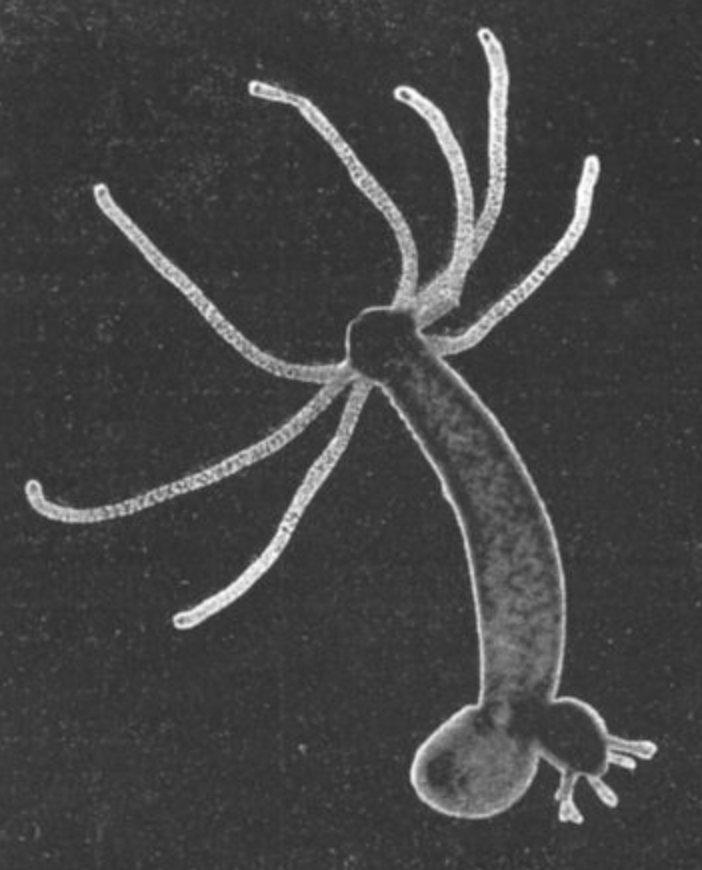
\includegraphics[scale=0.20]{hydra.png}
\end{figure}


\subsection{Nerve Nets}
\begin{itemize}
\item \textit{Hydra} have a diffuse nerve net rather than a CNS
\item Comprised of ganglia and a few types of sensory neurons
\item Once mature, a constant density gradient of neurons is maintained. Adults have no more than a few thousand neurons
\item Turns out nerve net is actually composed of non-overlapping circuits that correspond to specific sets of behaviors
\end{itemize}
\begin{figure}
\centering
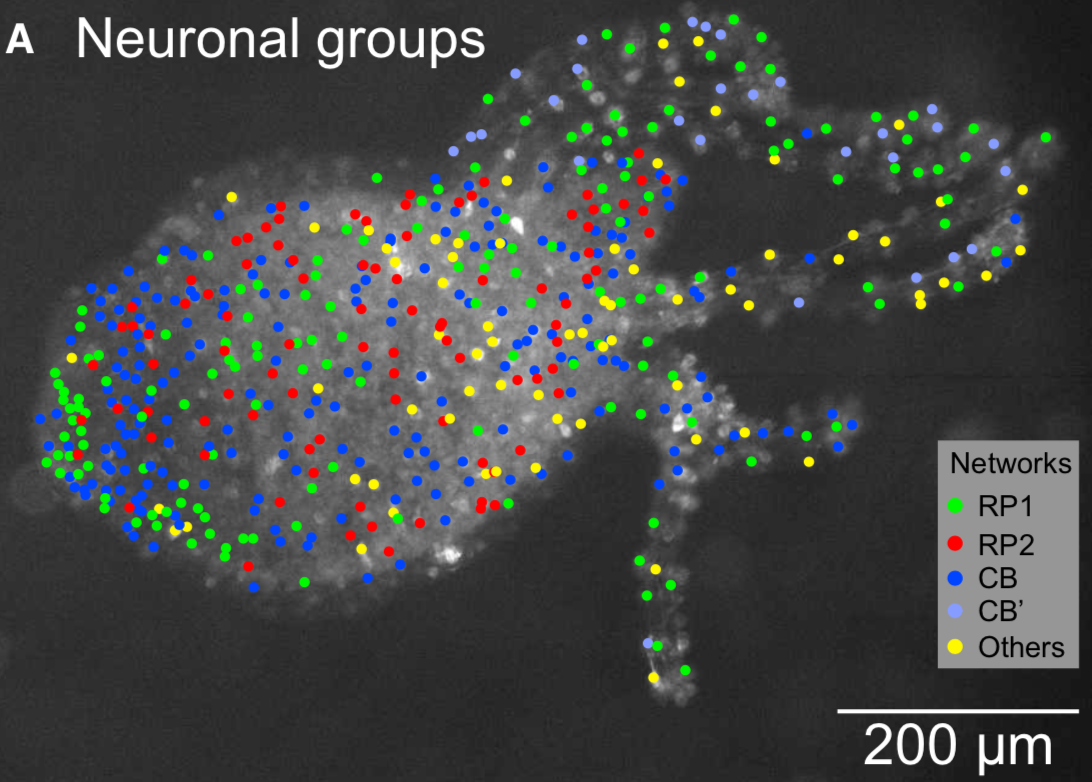
\includegraphics[scale=0.25]{hydra_map.png}
\end{figure}


\subsection{Separate Circuits}
\begin{itemize}
\item RP1 associated with longitudinal elongations
\item RP2 associated with radial contractions
\item CB associated with longitudinal contractions
\item STN associated with `nodding' behavior
\item RP1 and CB are antagonistic, no other interactions
\end{itemize}
\begin{figure}
\center
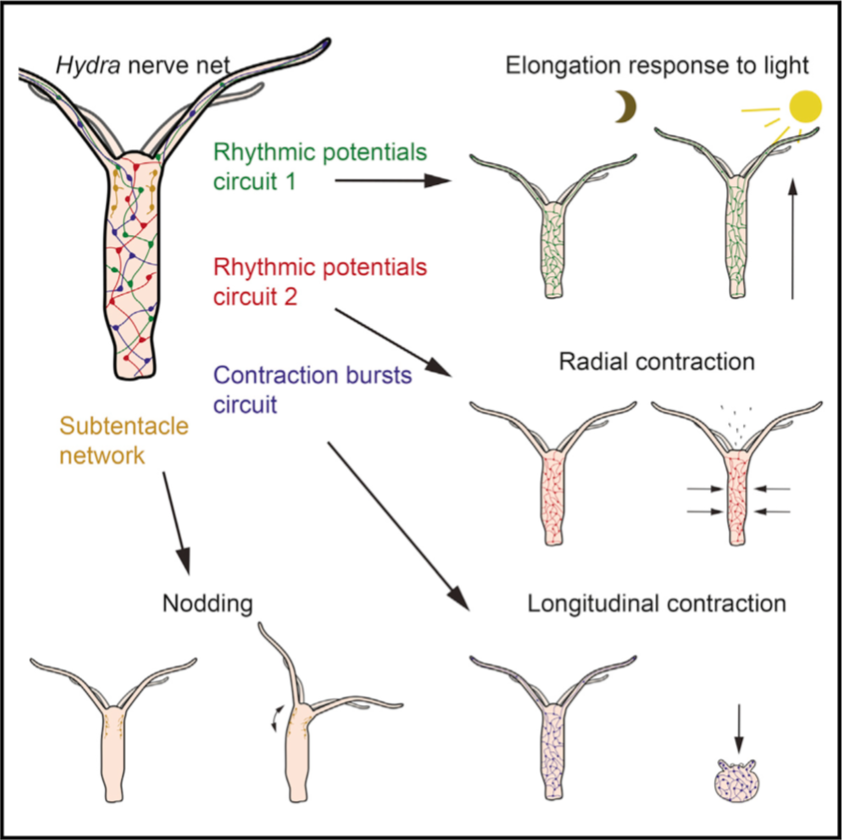
\includegraphics[scale=0.325]{hydra_movements.png}
\end{figure}


\subsection{Summary}
Advantages of \textit{Hydra} as a model organism:
\begin{itemize}
\item Very small size, so currents travel quickly and therefore the topology of the nerve net can be ignored at first approximation
\item Distinct behaviors appear to be controlled by distinct circuits, so analysis can be broken into many parts
\item Small amount of neurons and fixed neuronal density make simulation much easier
\end{itemize}


%%%%%%%%%%%%%%%%%%%%%%%%%%%%%%%%%%%%%%%%%%%%%%%%%%%%%%%%%%%%%%%%%%%%%%%%%
%%%%%%%%%%%%%%%%%%%%%%%%%%%%%%%%%%%%%%%%%%%%%%%%%%%%%%%%%%%%%%%%%%%%%%%%%
% Section 3
\section{Network Framework}
%%%%%%%%%%%%%%%%%%%%%%%%%%%%%%%%%%%%%%%%%%%%%%%%%%%%%%%%%%%%%%%%%%%%%%%%%
%%%%%%%%%%%%%%%%%%%%%%%%%%%%%%%%%%%%%%%%%%%%%%%%%%%%%%%%%%%%%%%%%%%%%%%%%

\subsection{Neuron Model}
\begin{itemize}
\item Leaky integrate-and-fire (LIF) model:
\begin{equation*}
\frac{dV_{m}}{dt}=\frac{1}{C_{m}}\left(-\frac{(V_{m}-V_{m}^{eq})}{R_{m}}+I_{ext}\right)
\end{equation*}
\item Computationally simpler than Hodgkin-Huxley
\item Models neuron as RC circuit with leak term
\item Doesn't explicitly specify spiking behavior or refractory period, but easy to implement using iterative ODE methods
\item Possible implementation:
\begin{figure}
\begin{verbatim}[fontsize=\scriptsize]
if V(t+1) > threshold:
   V(t)   <- spike
   V(t+1) <- hyperpolarize
if t in refractory period:
   V(t+1) <- hyperpolarize
\end{verbatim}
\end{figure}
\end{itemize}


\subsection{Antagonistic Neural Circuits}
\begin{itemize}
\item Assume each neuron of RP1 emits an inhibitory neurotransmitter $E_{RP1}$ when spiking, and similarly for CB with $E_{CB}$. Using concentrations, the model is:
\begin{align*}
\frac{dV_{RP1}}{dt}&=\frac{1}{C_{RP1}}\left(-\frac{(V_{RP1}-V_{RP1}^{eq})}{R_{RP1}}+I_{ext}\left(1-E_{CB}\right)\right)\\
\frac{dV_{CB}}{dt}&=\frac{1}{C_{CB}}\left(-\frac{(V_{CB}-V_{CB}^{eq})}{R_{CB}}+I_{ext}\left(1-E_{RP1}\right)\right)\\
\frac{dE_{RP1}}{dt}&=d_{RP1}E_{RP1}\hspace{2em}\frac{dE_{CB}}{dt}=d_{CB}E_{CB}
\end{align*}
\end{itemize}


\subsection{Antagonistic Neural Circuits (cont.)}
\begin{figure}
\center
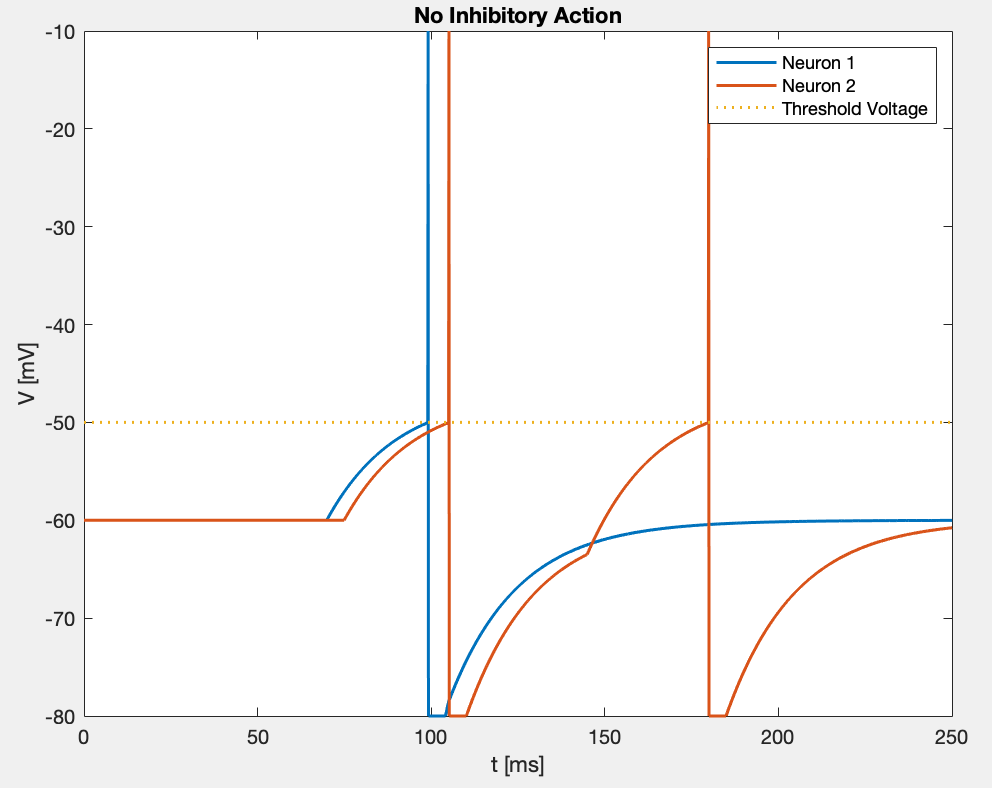
\includegraphics[scale=0.29]{no_inhib.png}\hspace{1em}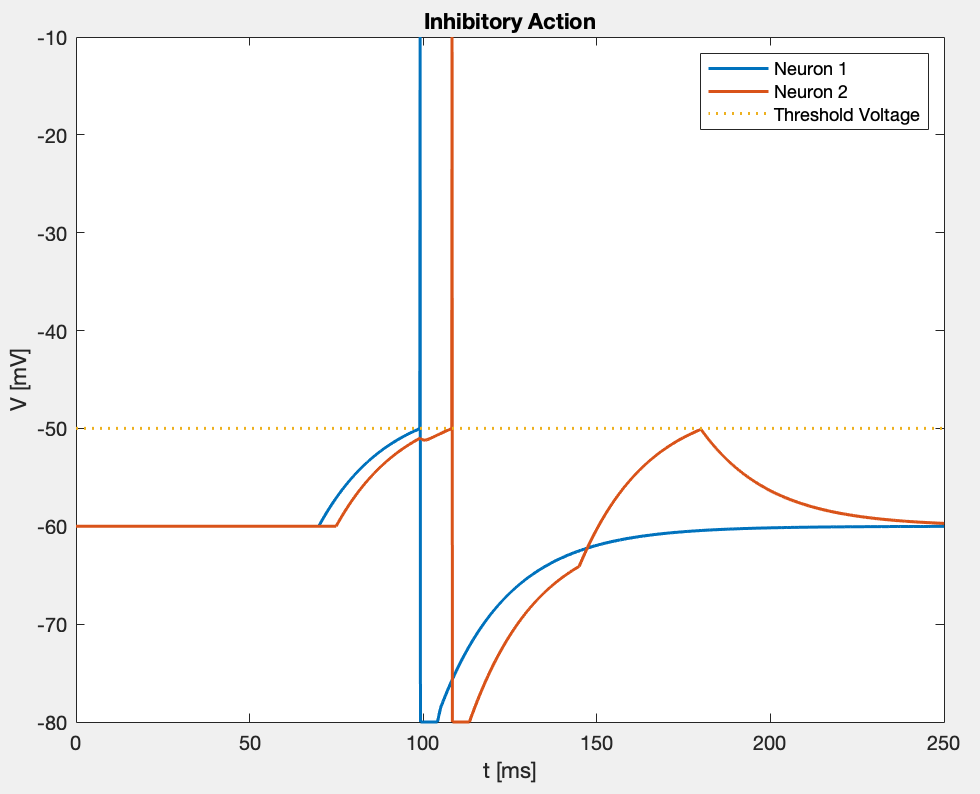
\includegraphics[scale=0.29]{inhib.png}
\caption{Simulation of two LIF neurons not acting on each other, and acting antagonistically, respectively. Input current is same in both simulations.}
\end{figure}



%%%%%%%%%%%%%%%%%%%%%%%%%%%%%%%%%%%%%%%%%%%%%%%%%%%%%%%%%%%%%%%%%%%%%%%%%
%%%%%%%%%%%%%%%%%%%%%%%%%%%%%%%%%%%%%%%%%%%%%%%%%%%%%%%%%%%%%%%%%%%%%%%%%
% Section 4
\section{Optimizations}
%%%%%%%%%%%%%%%%%%%%%%%%%%%%%%%%%%%%%%%%%%%%%%%%%%%%%%%%%%%%%%%%%%%%%%%%%
%%%%%%%%%%%%%%%%%%%%%%%%%%%%%%%%%%%%%%%%%%%%%%%%%%%%%%%%%%%%%%%%%%%%%%%%%

\subsection{SNN simplifications}
In our nerve network model, instead of fully simulating a continuous waveform for the state of the neuron, we keep track of the spikes at discrete timesteps instead. The primary advantage of spiked neural networks comes from the temporal coding, and this can be preserved with small enough discrete timesteps.\newline

One advantage of this approach is that the timestep size can be decreased if we find that information is not being encoded temporally as expected, or can be increased to save on processing power.


\subsection{Tensor Product Optimization}
We propose imposing non self-similar structure on the ``blank'' (before learning) nerve nets in the following fashion:\\
Where $H_1, H_2, \ldots, H_L$ are all graphs, we set  
$$ G = H_1 \otimes H_2 \otimes \cdots \otimes H_L $$
Where ``$\otimes$'' is the graph tensor product, equivalent to the matrix tensor product of the adjacency matrices of the graphs.\\
Tensor product $H \otimes K$ is equivalent to replacing every vertex in $H$ with a copy of $K$. Vertices have connections between them if their counterparts in either $H$ or $K$ have edges between them. This means a random walk on $H \otimes K$ can be simulated by a random walk on $H$ and $K$ at the same time.


\subsection{Tensor Product Optimization}
\begin{itemize}
    \item Note that the space required to store a graph as an adjacency matrix is $O(n^2)$ on the number of vertices
    \item If we assume $H_i$ has $n_i$ vertices, then we only require $ \sum_{i \in [1,L]} (n_i)^2 $ space to store the component graphs
    \item On the other hand, storing $G$ by itself requires space $ \prod_{i \in [1,L]} (n_i)^2 $
\end{itemize}


\subsection{Tensor Product Optimization, continued}
For large networks, the aforementioned size differences become very significant
\begin{itemize}
    \item Network with 5 layers of 100 neurons each will take only $5 \cdot 10^4$ units of memory to store by adjacency matrices
    \item the above 5-layer network describes a complex network with $100^{5}=10^{10}$ neurons that would take an adjacency matrix of size $10^{20}$ to describe
    \item assuming 1 byte memory per connection (very low estimate), the 5-layer network takes up about 50MB, while it's counterpart takes around a million TB to store directly. 
    \item Simulating and training this network is still computationally difficult, but space complexity  of is reduced
\end{itemize}


\subsection{Biological Motivation}
Making no assumptions about which genes affect the structure of the human brain, it is clearly impossible for the exact structure of the $>10^{10}$ neurons and $>10^{12}$ connections between them to be encoded in the mere $4 \cdot 10^{9}$ base pairs of the human genome. \\
\vspace{1em}
This tells us that there must be \textit{some} sort of repeated structure in most nerve networks. Granted, graph tensor products might not be the most realistic way to model this repeated structure, but we hope that our work is a small step in that direction.

% However, some structure is clearly present even before any meaningful information is learned. Instead, some general structure may be encoded genetically, and the ``details'' are filled in as the organism develops.


%%%%%%%%%%%%%%%%%%%%%%%%%%%%%%%%%%%%%%%%%%%%%%%%%%%%%%%%%%%%%%%%%%%%%%%%%
%%%%%%%%%%%%%%%%%%%%%%%%%%%%%%%%%%%%%%%%%%%%%%%%%%%%%%%%%%%%%%%%%%%%%%%%%
% Section 5
\section{Future Work}
%%%%%%%%%%%%%%%%%%%%%%%%%%%%%%%%%%%%%%%%%%%%%%%%%%%%%%%%%%%%%%%%%%%%%%%%%
%%%%%%%%%%%%%%%%%%%%%%%%%%%%%%%%%%%%%%%%%%%%%%%%%%%%%%%%%%%%%%%%%%%%%%%%%

\subsection{Short term goals}
\begin{itemize}
    \item Using existing data in the literature, finish creating out model of the \textit{Hydra} antagonistic nerve nets
    \item After creating a network that exhibits temporal signalling behavior, we hope to find the largest timestep $\Delta t$ that preserves this behavior. Knowing the largest possible timestep lets us run simulations faster, and grants insights about the nature of the temporal signaling.
    \item Extend the tensor product optimization to allow replacement of vertices in $H_i$ with different graphs, not just $H_{i+1}$. This will in theory allow the representation of a wider variety of graph patterns, notably allowing differences in local structure between larger regions
\end{itemize}


\subsection{Long term future work}
\begin{itemize}
    \item Train the framework described here for \textit{Hydra} on actual behavioral data from specimens. With sufficient training, the network described should be able to, in more or less real time, predict the behavior of \textit{Hydra} in response to external stimuli.
    \item Chemical signalling in the human brain plays a far more complex role than the relatively simple antagonistic networks in \textit{Hydra}. Extending our model to the human brain is far outside the scope of this project or modern technology, but perhaps some insight into chemical signalling systems in nerve nets can be gained.
    \item With more information about the nature of the temporal signalling, it may be possible to model the frequency domain instead of the time domain. This would be both easier for a human to read, and less computationally expensive.
\end{itemize}



\end{document}